\documentclass[a4paper]{book}
\usepackage{makeidx}
\usepackage{graphicx}
\usepackage{multicol}
\usepackage{float}
\usepackage{listings}
\usepackage{color}
\usepackage{ifthen}
\usepackage[table]{xcolor}
\usepackage{textcomp}
\usepackage{alltt}
\usepackage{ifpdf}
\ifpdf
\usepackage[pdftex,
            pagebackref=true,
            colorlinks=true,
            linkcolor=blue,
            unicode
           ]{hyperref}
\else
\usepackage[ps2pdf,
            pagebackref=true,
            colorlinks=true,
            linkcolor=blue,
            unicode
           ]{hyperref}
\usepackage{pspicture}
\fi
\usepackage[utf8]{inputenc}
\usepackage{mathptmx}
\usepackage[scaled=.90]{helvet}
\usepackage{courier}
\usepackage{doxygen}
\lstset{language=C++,inputencoding=utf8,basicstyle=\footnotesize,breaklines=true,breakatwhitespace=true,tabsize=8,numbers=left }
\makeindex
\setcounter{tocdepth}{3}
\renewcommand{\footrulewidth}{0.4pt}
\begin{document}
\hypersetup{pageanchor=false}
\begin{titlepage}
\vspace*{7cm}
\begin{center}
{\Large PG\_\-Btree \\[1ex]\large 0.1 }\\
\vspace*{1cm}
{\large Generated by Doxygen 1.7.3}\\
\vspace*{0.5cm}
{\small Wed Apr 4 2012 11:33:56}\\
\end{center}
\end{titlepage}
\clearemptydoublepage
\pagenumbering{roman}
\tableofcontents
\clearemptydoublepage
\pagenumbering{arabic}
\hypersetup{pageanchor=true}
\chapter{Class Index}
\section{Class Hierarchy}
This inheritance list is sorted roughly, but not completely, alphabetically:\begin{DoxyCompactList}
\item \contentsline{section}{BTree$<$ T, Cmp $>$}{\pageref{classBTree}}{}
\item \contentsline{section}{BTree$<$ T, Cmp $>$::generic\_\-iterator}{\pageref{classBTree_1_1generic__iterator}}{}
\begin{DoxyCompactList}
\item \contentsline{section}{BTree$<$ T, Cmp $>$::iterator}{\pageref{classBTree_1_1iterator}}{}
\item \contentsline{section}{BTree$<$ T, Cmp $>$::reverse\_\-iterator}{\pageref{classBTree_1_1reverse__iterator}}{}
\end{DoxyCompactList}
\item \contentsline{section}{Node$<$ T, Cmp $>$}{\pageref{classNode}}{}
\end{DoxyCompactList}

\chapter{Class Index}
\section{Class List}
Here are the classes, structs, unions and interfaces with brief descriptions:\begin{DoxyCompactList}
\item\contentsline{section}{\hyperlink{classBTree}{BTree$<$ T, Cmp $>$} (Conainter class. Store Nodes in a Tree )}{\pageref{classBTree}}{}
\item\contentsline{section}{\hyperlink{classBTree_1_1generic__iterator}{BTree$<$ T, Cmp $>$::generic\_\-iterator} }{\pageref{classBTree_1_1generic__iterator}}{}
\item\contentsline{section}{\hyperlink{classBTree_1_1iterator}{BTree$<$ T, Cmp $>$::iterator} }{\pageref{classBTree_1_1iterator}}{}
\item\contentsline{section}{\hyperlink{classNode}{Node$<$ T, Cmp $>$} (\hyperlink{classBTree}{BTree} \hyperlink{classNode}{Node}. Contains Elements/Keys )}{\pageref{classNode}}{}
\item\contentsline{section}{\hyperlink{classBTree_1_1reverse__iterator}{BTree$<$ T, Cmp $>$::reverse\_\-iterator} }{\pageref{classBTree_1_1reverse__iterator}}{}
\end{DoxyCompactList}

\chapter{Class Documentation}
\hypertarget{classBArbre}{
\section{BArbre$<$ T $>$ Class Template Reference}
\label{classBArbre}\index{BArbre@{BArbre}}
}
\subsection*{Classes}
\begin{DoxyCompactItemize}
\item 
class \hyperlink{classBArbre_1_1generic__iterator}{generic\_\-iterator}
\item 
class \hyperlink{classBArbre_1_1iterator}{iterator}
\item 
class \hyperlink{classBArbre_1_1reverse__iterator}{reverse\_\-iterator}
\end{DoxyCompactItemize}
\subsection*{Public Member Functions}
\begin{DoxyCompactItemize}
\item 
\hypertarget{classBArbre_abf97ee99962ab0fd16080db5c3b1f02f}{
{\bfseries BArbre} (int lower=2, int upper=-\/1)}
\label{classBArbre_abf97ee99962ab0fd16080db5c3b1f02f}

\item 
\hypertarget{classBArbre_a0612c34605cbe9236e447910a96d9f94}{
void {\bfseries ajouterElement} (const T \&element)}
\label{classBArbre_a0612c34605cbe9236e447910a96d9f94}

\item 
\hypertarget{classBArbre_afb35c6904f78d12510b7e763d31ef1f7}{
int {\bfseries supprimerElement} (T element)}
\label{classBArbre_afb35c6904f78d12510b7e763d31ef1f7}

\item 
\hypertarget{classBArbre_a54d1be427a621ce93d74eef55e8b1fae}{
T {\bfseries chercherElement} (const T \&element)}
\label{classBArbre_a54d1be427a621ce93d74eef55e8b1fae}

\item 
\hypertarget{classBArbre_a1b6e56dfd6fdb8af661c208ae9d645be}{
\hyperlink{classNoeud}{Noeud}$<$ T $>$ $\ast$ {\bfseries chercherElementN} (const T \&element)}
\label{classBArbre_a1b6e56dfd6fdb8af661c208ae9d645be}

\item 
\hypertarget{classBArbre_a3a8ad2d9d5a3fd60c678d79db29e4298}{
void {\bfseries draw} (std::ostream \&flux) const }
\label{classBArbre_a3a8ad2d9d5a3fd60c678d79db29e4298}

\item 
\hypertarget{classBArbre_ad22b69148af1ece9b1a1d47773862771}{
std::vector$<$ \hyperlink{classNoeud}{Noeud}$<$ T $>$ $\ast$ $>$ {\bfseries addToNode} (\hyperlink{classNoeud}{Noeud}$<$ T $>$ $\ast$node, const T \&element)}
\label{classBArbre_ad22b69148af1ece9b1a1d47773862771}

\item 
\hypertarget{classBArbre_a38bee8f1d2656cfe95c72fbc5b2c7e01}{
std::vector$<$ \hyperlink{classNoeud}{Noeud}$<$ T $>$ $\ast$ $>$ {\bfseries splitNode} (\hyperlink{classNoeud}{Noeud}$<$ T $>$ $\ast$node)}
\label{classBArbre_a38bee8f1d2656cfe95c72fbc5b2c7e01}

\item 
\hypertarget{classBArbre_ad6c3166fd15b5ee9ff3b82ab36c9c5f2}{
std::vector$<$ \hyperlink{classNoeud}{Noeud}$<$ T $>$ $\ast$ $>$ {\bfseries balanceNode} (\hyperlink{classNoeud}{Noeud}$<$ T $>$ $\ast$node)}
\label{classBArbre_ad6c3166fd15b5ee9ff3b82ab36c9c5f2}

\item 
\hypertarget{classBArbre_ade188700cafaaba30bafa917ce5673e2}{
void {\bfseries mergeNodes} (\hyperlink{classNoeud}{Noeud}$<$ T $>$ $\ast$targetNode, \hyperlink{classNoeud}{Noeud}$<$ T $>$ $\ast$sourceNode)}
\label{classBArbre_ade188700cafaaba30bafa917ce5673e2}

\item 
\hypertarget{classBArbre_a19f8e4a34c3548815e12238aa8bbc452}{
int {\bfseries removeFromNode} (\hyperlink{classNoeud}{Noeud}$<$ T $>$ $\ast$node, const T \&element)}
\label{classBArbre_a19f8e4a34c3548815e12238aa8bbc452}

\item 
\hypertarget{classBArbre_a9238a234e0fe293016cff6357854bfd5}{
int {\bfseries size} ()}
\label{classBArbre_a9238a234e0fe293016cff6357854bfd5}

\item 
\hypertarget{classBArbre_a6602cf7c0f6a7f3a7e8c27917e4f54c8}{
\hyperlink{classNoeud}{Noeud}$<$ T $>$ $\ast$ {\bfseries getRootNode} ()}
\label{classBArbre_a6602cf7c0f6a7f3a7e8c27917e4f54c8}

\item 
\hypertarget{classBArbre_abc6be6012c8d0ff48cdf6e67337de03e}{
\hyperlink{classBArbre_1_1iterator}{iterator} {\bfseries begin} ()}
\label{classBArbre_abc6be6012c8d0ff48cdf6e67337de03e}

\item 
\hypertarget{classBArbre_ad0de78fea4611cc9a6f4d2992a6fc899}{
\hyperlink{classBArbre_1_1reverse__iterator}{reverse\_\-iterator} {\bfseries rbegin} ()}
\label{classBArbre_ad0de78fea4611cc9a6f4d2992a6fc899}

\item 
\hypertarget{classBArbre_a09d28b28bf01b215b8dbe7f9a0a5a55b}{
\hyperlink{classBArbre_1_1iterator}{iterator} {\bfseries end} ()}
\label{classBArbre_a09d28b28bf01b215b8dbe7f9a0a5a55b}

\item 
\hypertarget{classBArbre_a0190a3b190f9dac6bfeda51f69732f20}{
\hyperlink{classBArbre_1_1reverse__iterator}{reverse\_\-iterator} {\bfseries rend} ()}
\label{classBArbre_a0190a3b190f9dac6bfeda51f69732f20}

\item 
\hypertarget{classBArbre_a572ecf896ce181b96ec235a559a50017}{
\hyperlink{classBArbre_1_1iterator}{iterator} {\bfseries root} ()}
\label{classBArbre_a572ecf896ce181b96ec235a559a50017}

\end{DoxyCompactItemize}
\subsection*{Public Attributes}
\begin{DoxyCompactItemize}
\item 
\hypertarget{classBArbre_a3d3ca78a7094e8f5c32cd870b1b43d32}{
int {\bfseries \_\-dbg}}
\label{classBArbre_a3d3ca78a7094e8f5c32cd870b1b43d32}

\end{DoxyCompactItemize}
\subsubsection*{template$<$typename T$>$ class BArbre$<$ T $>$}



The documentation for this class was generated from the following file:\begin{DoxyCompactItemize}
\item 
/media/Programmes/Dropbox/Univ nantes -\/ Master 1 ALMA/ProgGenerative/projet\_\-tp/Arbre\_\-b/src/BArbre.h\end{DoxyCompactItemize}

\hypertarget{classBArbre_1_1generic__iterator}{
\section{BArbre$<$ T $>$::generic\_\-iterator Class Reference}
\label{classBArbre_1_1generic__iterator}\index{BArbre::generic\_\-iterator@{BArbre::generic\_\-iterator}}
}
Inheritance diagram for BArbre$<$ T $>$::generic\_\-iterator:\begin{figure}[H]
\begin{center}
\leavevmode
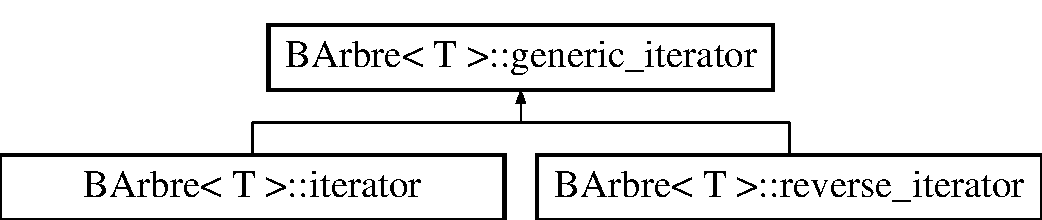
\includegraphics[height=2.000000cm]{classBArbre_1_1generic__iterator}
\end{center}
\end{figure}
\subsection*{Public Member Functions}
\begin{DoxyCompactItemize}
\item 
\hypertarget{classBArbre_1_1generic__iterator_abea43f33130b541d4c713c6bb56a5618}{
{\bfseries generic\_\-iterator} (\hyperlink{classBArbre}{BArbre}$<$ T $>$ $\ast$a, bool ended=false)}
\label{classBArbre_1_1generic__iterator_abea43f33130b541d4c713c6bb56a5618}

\item 
\hypertarget{classBArbre_1_1generic__iterator_aa3e1024170c9dfd01f22c6c89e862fe0}{
const T \& {\bfseries operator$\ast$} () const }
\label{classBArbre_1_1generic__iterator_aa3e1024170c9dfd01f22c6c89e862fe0}

\item 
\hypertarget{classBArbre_1_1generic__iterator_a290bda0be491b32f597c97d45836fc71}{
bool {\bfseries operator!=} (const \hyperlink{classBArbre}{BArbre}$<$ T $>$::\hyperlink{classBArbre_1_1generic__iterator}{generic\_\-iterator} \&itCmp) const }
\label{classBArbre_1_1generic__iterator_a290bda0be491b32f597c97d45836fc71}

\item 
\hypertarget{classBArbre_1_1generic__iterator_af2cc8115fa807f68d2a26d5693f15192}{
void {\bfseries operator++} (int ba)}
\label{classBArbre_1_1generic__iterator_af2cc8115fa807f68d2a26d5693f15192}

\item 
\hypertarget{classBArbre_1_1generic__iterator_acd1321a0f0d3ef360fd4df583b73eabc}{
void {\bfseries operator-\/-\/} (int ba)}
\label{classBArbre_1_1generic__iterator_acd1321a0f0d3ef360fd4df583b73eabc}

\item 
\hypertarget{classBArbre_1_1generic__iterator_a41ddc93c8700ac2de8b2e582df1472e5}{
bool {\bfseries operator$<$} (const \hyperlink{classBArbre}{BArbre}$<$ T $>$::\hyperlink{classBArbre_1_1generic__iterator}{generic\_\-iterator} \&itCmp)}
\label{classBArbre_1_1generic__iterator_a41ddc93c8700ac2de8b2e582df1472e5}

\item 
\hypertarget{classBArbre_1_1generic__iterator_ab3fd77d303ebb9ecefb73705662a2334}{
virtual void {\bfseries next} ()=0}
\label{classBArbre_1_1generic__iterator_ab3fd77d303ebb9ecefb73705662a2334}

\item 
\hypertarget{classBArbre_1_1generic__iterator_a1553fe665f6aac5217bc9b7fc2d5646f}{
virtual void {\bfseries previous} ()=0}
\label{classBArbre_1_1generic__iterator_a1553fe665f6aac5217bc9b7fc2d5646f}

\item 
\hypertarget{classBArbre_1_1generic__iterator_a20c07b11acf0f1cb3b736b6ff207ed54}{
virtual void {\bfseries toFirstElement} ()=0}
\label{classBArbre_1_1generic__iterator_a20c07b11acf0f1cb3b736b6ff207ed54}

\item 
\hypertarget{classBArbre_1_1generic__iterator_a4d24444d3d847e09d129776a7eb9a613}{
\hyperlink{classBArbre}{BArbre}$<$ T $>$::\hyperlink{classBArbre_1_1generic__iterator}{generic\_\-iterator} {\bfseries operator+} (int inc) const }
\label{classBArbre_1_1generic__iterator_a4d24444d3d847e09d129776a7eb9a613}

\item 
\hypertarget{classBArbre_1_1generic__iterator_a9e25f7baedfc09ccf63704ed80816d27}{
void {\bfseries toParentR} ()}
\label{classBArbre_1_1generic__iterator_a9e25f7baedfc09ccf63704ed80816d27}

\item 
\hypertarget{classBArbre_1_1generic__iterator_ab6514b46fcfc89044f23098b4fc2926b}{
void {\bfseries toParentL} ()}
\label{classBArbre_1_1generic__iterator_ab6514b46fcfc89044f23098b4fc2926b}

\end{DoxyCompactItemize}
\subsection*{Protected Member Functions}
\begin{DoxyCompactItemize}
\item 
\hypertarget{classBArbre_1_1generic__iterator_ac2747857dc30b31b344a57e58c26b38c}{
void {\bfseries toLeft} ()}
\label{classBArbre_1_1generic__iterator_ac2747857dc30b31b344a57e58c26b38c}

\item 
\hypertarget{classBArbre_1_1generic__iterator_a722d723e35a12756bb3307e51286cc7c}{
void {\bfseries toRight} ()}
\label{classBArbre_1_1generic__iterator_a722d723e35a12756bb3307e51286cc7c}

\item 
\hypertarget{classBArbre_1_1generic__iterator_a416a7ba21fe44553da54d4c6f488d663}{
void {\bfseries toRightIndex} ()}
\label{classBArbre_1_1generic__iterator_a416a7ba21fe44553da54d4c6f488d663}

\item 
\hypertarget{classBArbre_1_1generic__iterator_a8d675e482c5a4a178ca2cf0c943e5913}{
void {\bfseries toLeftIndex} ()}
\label{classBArbre_1_1generic__iterator_a8d675e482c5a4a178ca2cf0c943e5913}

\item 
\hypertarget{classBArbre_1_1generic__iterator_a3fe779ec1f1bb330ef26a0e754f774e4}{
bool {\bfseries ended} () const }
\label{classBArbre_1_1generic__iterator_a3fe779ec1f1bb330ef26a0e754f774e4}

\end{DoxyCompactItemize}
\subsection*{Protected Attributes}
\begin{DoxyCompactItemize}
\item 
\hypertarget{classBArbre_1_1generic__iterator_aa36f57491e6c5024ea0673e6ae123ecd}{
\hyperlink{classBArbre}{BArbre}$<$ T $>$ $\ast$ {\bfseries \_\-a}}
\label{classBArbre_1_1generic__iterator_aa36f57491e6c5024ea0673e6ae123ecd}

\item 
\hypertarget{classBArbre_1_1generic__iterator_ae20f521a11ce3c0f082c36ea3ba77164}{
\hyperlink{classNoeud}{Noeud}$<$ T $>$ $\ast$ {\bfseries \_\-current\_\-node}}
\label{classBArbre_1_1generic__iterator_ae20f521a11ce3c0f082c36ea3ba77164}

\item 
\hypertarget{classBArbre_1_1generic__iterator_a9150be6f68442eca99ddd8687f19c53b}{
int {\bfseries \_\-current\_\-index}}
\label{classBArbre_1_1generic__iterator_a9150be6f68442eca99ddd8687f19c53b}

\item 
\hypertarget{classBArbre_1_1generic__iterator_ae46ae1021d2e230d26893931e27060b4}{
bool {\bfseries \_\-ended}}
\label{classBArbre_1_1generic__iterator_ae46ae1021d2e230d26893931e27060b4}

\end{DoxyCompactItemize}
\subsubsection*{template$<$typename T$>$ class BArbre$<$ T $>$::generic\_\-iterator}



The documentation for this class was generated from the following file:\begin{DoxyCompactItemize}
\item 
/media/Programmes/Dropbox/Univ nantes -\/ Master 1 ALMA/ProgGenerative/projet\_\-tp/Arbre\_\-b/src/BArbre\_\-generic\_\-iterator.h\end{DoxyCompactItemize}

\hypertarget{classBArbre_1_1iterator}{
\section{BArbre$<$ T $>$::iterator Class Reference}
\label{classBArbre_1_1iterator}\index{BArbre::iterator@{BArbre::iterator}}
}
Inheritance diagram for BArbre$<$ T $>$::iterator:\begin{figure}[H]
\begin{center}
\leavevmode
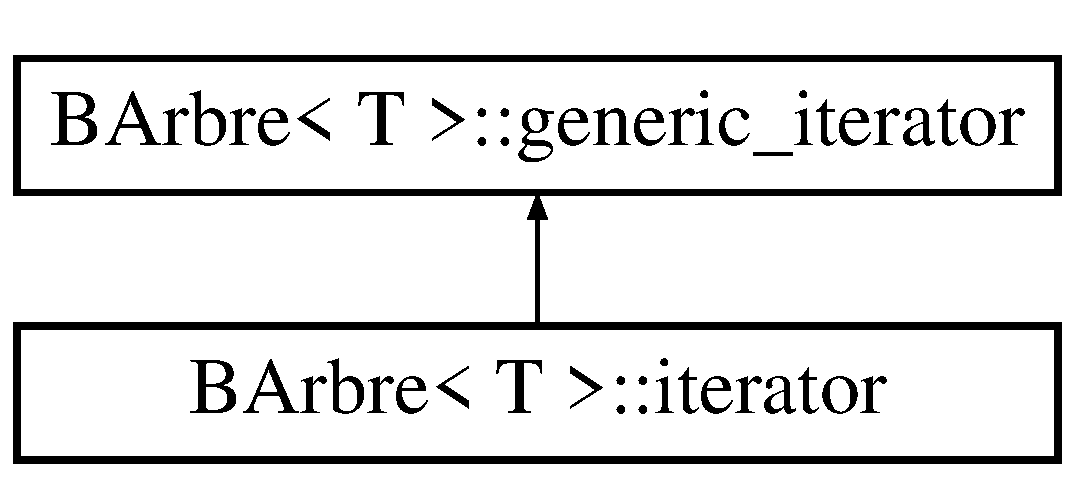
\includegraphics[height=2.000000cm]{classBArbre_1_1iterator}
\end{center}
\end{figure}
\subsection*{Public Member Functions}
\begin{DoxyCompactItemize}
\item 
\hypertarget{classBArbre_1_1iterator_adf85f21458befaef3c185047e25c2d8b}{
{\bfseries iterator} (\hyperlink{classBArbre}{BArbre}$<$ T $>$ $\ast$a, bool ended=false)}
\label{classBArbre_1_1iterator_adf85f21458befaef3c185047e25c2d8b}

\item 
\hypertarget{classBArbre_1_1iterator_add128dc1221f82dc5438be9fba6e7375}{
virtual void {\bfseries previous} ()}
\label{classBArbre_1_1iterator_add128dc1221f82dc5438be9fba6e7375}

\item 
\hypertarget{classBArbre_1_1iterator_ad311970e22af2f3ac601a2411546e109}{
virtual void {\bfseries next} ()}
\label{classBArbre_1_1iterator_ad311970e22af2f3ac601a2411546e109}

\item 
\hypertarget{classBArbre_1_1iterator_a88e263613e498505517be010fab57132}{
virtual void {\bfseries toFirstElement} ()}
\label{classBArbre_1_1iterator_a88e263613e498505517be010fab57132}

\item 
\hypertarget{classBArbre_1_1iterator_a35d2d27919a4cd5005290c7b1270155f}{
{\bfseries iterator} (\hyperlink{classBArbre}{BarbreG} $\ast$a, \hyperlink{classNoeud}{NoeudG} $\ast$n)}
\label{classBArbre_1_1iterator_a35d2d27919a4cd5005290c7b1270155f}

\item 
\hypertarget{classBArbre_1_1iterator_a0308ab6a130eb44d6172f43d4665c333}{
const T \& {\bfseries operator$\ast$} () const }
\label{classBArbre_1_1iterator_a0308ab6a130eb44d6172f43d4665c333}

\item 
\hypertarget{classBArbre_1_1iterator_a4c386a507353fe56911bf81d0a577db6}{
void {\bfseries operator++} (int i)}
\label{classBArbre_1_1iterator_a4c386a507353fe56911bf81d0a577db6}

\end{DoxyCompactItemize}
\subsubsection*{template$<$typename T$>$ class BArbre$<$ T $>$::iterator}



The documentation for this class was generated from the following files:\begin{DoxyCompactItemize}
\item 
/media/Programmes/Dropbox/Univ nantes -\/ Master 1 ALMA/ProgGenerative/projet\_\-tp/Arbre\_\-b/src/BArbre\_\-iterator.h\item 
/media/Programmes/Dropbox/Univ nantes -\/ Master 1 ALMA/ProgGenerative/projet\_\-tp/Arbre\_\-b/src/TestIter.h\end{DoxyCompactItemize}

\hypertarget{classNoeud}{
\section{Noeud$<$ T $>$ Class Template Reference}
\label{classNoeud}\index{Noeud@{Noeud}}
}
\subsection*{Public Member Functions}
\begin{DoxyCompactItemize}
\item 
\hypertarget{classNoeud_a7a68d0e206df13194413328fa431812e}{
{\bfseries Noeud} (\hyperlink{classNoeud}{Noeud}$<$ T $>$ $\ast$parent)}
\label{classNoeud_a7a68d0e206df13194413328fa431812e}

\item 
\hypertarget{classNoeud_a35239304a73f207562c18518dbf1e099}{
T {\bfseries getElement} (int i)}
\label{classNoeud_a35239304a73f207562c18518dbf1e099}

\item 
\hypertarget{classNoeud_accd8d04f9486008c19e632fe7e7ab092}{
int {\bfseries addElement} (T elt)}
\label{classNoeud_accd8d04f9486008c19e632fe7e7ab092}

\item 
\hypertarget{classNoeud_a3dd8653eacafccb54af61b7e10c696b8}{
int {\bfseries delElement} (const T \&element)}
\label{classNoeud_a3dd8653eacafccb54af61b7e10c696b8}

\item 
\hypertarget{classNoeud_a1a212caae417e8c986c7747263781519}{
std::vector$<$ T $>$ \& {\bfseries getElements} ()}
\label{classNoeud_a1a212caae417e8c986c7747263781519}

\item 
\hypertarget{classNoeud_a17b8932e392231d3b8064e53f96f11ee}{
int {\bfseries linkSon} (\hyperlink{classNoeud}{Noeud}$<$ T $>$ $\ast$node, int index=-\/1)}
\label{classNoeud_a17b8932e392231d3b8064e53f96f11ee}

\item 
\hypertarget{classNoeud_a83aecc420674abe5e7eb87be5de777bc}{
void {\bfseries unlinkSon} (\hyperlink{classNoeud}{Noeud}$<$ T $>$ $\ast$node)}
\label{classNoeud_a83aecc420674abe5e7eb87be5de777bc}

\item 
\hypertarget{classNoeud_aa530f295f3e72312e40a97571d40be61}{
std::vector$<$ \hyperlink{classNoeud}{Noeud}$<$ T $>$ $\ast$ $>$ \& {\bfseries getSons} ()}
\label{classNoeud_aa530f295f3e72312e40a97571d40be61}

\item 
\hypertarget{classNoeud_a7f0b92d936783852dd8f6005c0af46c1}{
void {\bfseries setParent} (\hyperlink{classNoeud}{Noeud}$<$ T $>$ $\ast$parent)}
\label{classNoeud_a7f0b92d936783852dd8f6005c0af46c1}

\item 
\hypertarget{classNoeud_a45b167fcea2f17f982c78700dfefe200}{
\hyperlink{classNoeud}{Noeud}$<$ T $>$ $\ast$ {\bfseries getParent} ()}
\label{classNoeud_a45b167fcea2f17f982c78700dfefe200}

\item 
\hypertarget{classNoeud_ad0d9bb9321ec052b84bc2b0ad0d3cd2f}{
bool {\bfseries contains} (const T \&elt)}
\label{classNoeud_ad0d9bb9321ec052b84bc2b0ad0d3cd2f}

\item 
\hypertarget{classNoeud_a2027d0f848391fb0b7aa0e599568aa95}{
bool {\bfseries isLeaf} ()}
\label{classNoeud_a2027d0f848391fb0b7aa0e599568aa95}

\item 
\hypertarget{classNoeud_abe2105490466f57d202308123fae8726}{
bool {\bfseries isOverflowing} (int size)}
\label{classNoeud_abe2105490466f57d202308123fae8726}

\item 
\hypertarget{classNoeud_aec41238cb00861543f2d819a706d82b0}{
bool {\bfseries isUnderflowing} (int min\_\-size)}
\label{classNoeud_aec41238cb00861543f2d819a706d82b0}

\item 
\hypertarget{classNoeud_a458ef7ea7113a03e3cdf562ca75a3a0f}{
int {\bfseries getElementPosition} (const T \&element)}
\label{classNoeud_a458ef7ea7113a03e3cdf562ca75a3a0f}

\item 
\hypertarget{classNoeud_a34ec8dfd905946d3a55e7ddc0a3fd07d}{
\hyperlink{classNoeud}{Noeud}$<$ T $>$ $\ast$ {\bfseries leftmostLeaf} ()}
\label{classNoeud_a34ec8dfd905946d3a55e7ddc0a3fd07d}

\item 
\hypertarget{classNoeud_acb5eef9cce35d271078628be447e7bd7}{
\hyperlink{classNoeud}{Noeud}$<$ T $>$ $\ast$ {\bfseries rightmostLeaf} ()}
\label{classNoeud_acb5eef9cce35d271078628be447e7bd7}

\item 
\hypertarget{classNoeud_a976a7fcb72e63237c9f3c8f85ddb820d}{
int {\bfseries element\_\-count} ()}
\label{classNoeud_a976a7fcb72e63237c9f3c8f85ddb820d}

\item 
\hypertarget{classNoeud_a8f9a238c0455368945aeaa531bed9228}{
int {\bfseries getSonPosition} (\hyperlink{classNoeud}{Noeud}$<$ T $>$ $\ast$son)}
\label{classNoeud_a8f9a238c0455368945aeaa531bed9228}

\item 
\hypertarget{classNoeud_aa4d7f22c303c08ce8848087e3594aaa6}{
int {\bfseries size} ()}
\label{classNoeud_aa4d7f22c303c08ce8848087e3594aaa6}

\item 
\hypertarget{classNoeud_a14192544a21e81363cbf3ed6a58aa28b}{
void {\bfseries draw} (std::ostream \&flux) const }
\label{classNoeud_a14192544a21e81363cbf3ed6a58aa28b}

\end{DoxyCompactItemize}
\subsubsection*{template$<$typename T$>$ class Noeud$<$ T $>$}



The documentation for this class was generated from the following file:\begin{DoxyCompactItemize}
\item 
/media/Programmes/Dropbox/Univ nantes -\/ Master 1 ALMA/ProgGenerative/projet\_\-tp/Arbre\_\-b/src/Noeud.h\end{DoxyCompactItemize}

\hypertarget{classBArbre_1_1reverse__iterator}{
\section{BArbre$<$ T $>$::reverse\_\-iterator Class Reference}
\label{classBArbre_1_1reverse__iterator}\index{BArbre::reverse\_\-iterator@{BArbre::reverse\_\-iterator}}
}
Inheritance diagram for BArbre$<$ T $>$::reverse\_\-iterator:\begin{figure}[H]
\begin{center}
\leavevmode
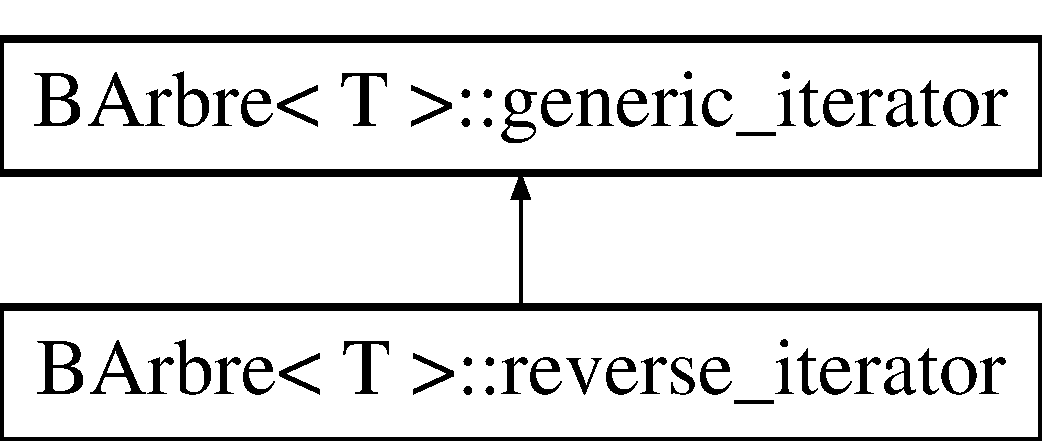
\includegraphics[height=2.000000cm]{classBArbre_1_1reverse__iterator}
\end{center}
\end{figure}
\subsection*{Public Member Functions}
\begin{DoxyCompactItemize}
\item 
\hypertarget{classBArbre_1_1reverse__iterator_a0970e2dc74d754fd589001cc11073d15}{
{\bfseries reverse\_\-iterator} (\hyperlink{classBArbre}{BArbre}$<$ T $>$ $\ast$a, bool ended=false)}
\label{classBArbre_1_1reverse__iterator_a0970e2dc74d754fd589001cc11073d15}

\item 
\hypertarget{classBArbre_1_1reverse__iterator_a154ec414876ae73d6ade14af3573dfae}{
virtual void {\bfseries previous} ()}
\label{classBArbre_1_1reverse__iterator_a154ec414876ae73d6ade14af3573dfae}

\item 
\hypertarget{classBArbre_1_1reverse__iterator_a1ec32209dbbb17b83d63db39a4a3ea98}{
virtual void {\bfseries next} ()}
\label{classBArbre_1_1reverse__iterator_a1ec32209dbbb17b83d63db39a4a3ea98}

\item 
\hypertarget{classBArbre_1_1reverse__iterator_a64e48f58c7111d7c2dbde5eaf61806d9}{
virtual void {\bfseries toFirstElement} ()}
\label{classBArbre_1_1reverse__iterator_a64e48f58c7111d7c2dbde5eaf61806d9}

\end{DoxyCompactItemize}
\subsubsection*{template$<$typename T$>$ class BArbre$<$ T $>$::reverse\_\-iterator}



The documentation for this class was generated from the following file:\begin{DoxyCompactItemize}
\item 
/media/Programmes/Dropbox/Univ nantes -\/ Master 1 ALMA/ProgGenerative/projet\_\-tp/Arbre\_\-b/src/BArbre\_\-reverse\_\-iterator.h\end{DoxyCompactItemize}

\printindex
\end{document}
